%%%%%% -*- Coding: utf-8-unix; Mode: latex

\documentclass[polish]{aghengthesis}
%\documentclass[english]{aghengthesis} %dla pracy w języku angielskim. Uwaga, w przypadku strony tytułowej zmiana języka dotyczy tylko kolejności wersji językowych tytułu pracy. 

\usepackage{tgtermes}
\usepackage[T1]{fontenc}
\usepackage{polski}
\usepackage[utf8]{inputenc}
\usepackage{url}
\usepackage{subfigure}
\usepackage{tabularx}
\usepackage{ragged2e}
\usepackage{booktabs}
\usepackage{multirow}
\usepackage{grffile}
\usepackage{indentfirst}
\usepackage{caption}
\usepackage{listings}
\usepackage[ruled,linesnumbered,lined]{algorithm2e}
\usepackage[bookmarks=false]{hyperref}
\usepackage{float}
\hypersetup{colorlinks,
  linkcolor=blue,
  citecolor=blue,
  urlcolor=blue}

\usepackage[svgnames]{xcolor}
\usepackage{inconsolata}

\usepackage{csquotes}
\DeclareQuoteStyle[quotes]{polish}
  {\quotedblbase}
  {\textquotedblright}
  [0.05em]
  {\quotesinglbase}
  {\fixligatures\textquoteright}
\DeclareQuoteAlias[quotes]{polish}{polish}

\usepackage[nottoc]{tocbibind}

\usepackage[
style=numeric,
sorting=nyt,
isbn=false,
doi=true,
url=true,
backref=false,
backrefstyle=none,
maxnames=10,
giveninits=true,
abbreviate=true,
defernumbers=false,
backend=biber]{biblatex}
\addbibresource{bibliografia.bib}

\lstset{
    %language=Python, %% PHP, C, Java, etc.
    basicstyle=\ttfamily\footnotesize,
    backgroundcolor=\color{gray!5},
    commentstyle=\it\color{Green},
    keywordstyle=\color{Red},
    stringstyle=\color{Blue},
    numberstyle=\tiny\color{Black},    
    % morekeywords={TestKeyword},
    % mathescape=true,
    escapeinside=`',
    frame=single, %shadowbox, 
    tabsize=2,
    rulecolor=\color{black!30},
    title=\lstname,
    breaklines=true,
    breakatwhitespace=true,
    framextopmargin=2pt,
    framexbottommargin=2pt,
    extendedchars=false,
    captionpos=b,
    abovecaptionskip=5pt,
    keepspaces=true,            
    numbers=left,                    
    numbersep=5pt,                  
    showspaces=false,                
    showstringspaces=false,
    showtabs=false,
    tabsize=2
  }

\SetAlgorithmName{\LangAlgorithm}{\LangAlgorithmRef}{\LangListOfAlgorithms}
\newcommand{\listofalgorithmes}{\tocfile{\listalgorithmcfname}{loa}}

\renewcommand{\lstlistingname}{\LangListing}
\renewcommand\lstlistlistingname{\LangListOfListings}

\renewcommand{\lstlistoflistings}{\begingroup
\tocfile{\lstlistlistingname}{lol}
\endgroup}

% Definicje nowych rodzajów kolumn w tabeli
\newcolumntype{Y}{>{\small\centering\arraybackslash}X}
%\newcolumntype{b}{>{\hsize=1.6\hsize}Y}
%\newcolumntype{m}{>{\hsize=.6\hsize}Y}
%\newcolumntype{s}{>{\hsize=.4\hsize}Y}

\captionsetup[figure]{skip=5pt,position=bottom}
\captionsetup[table]{skip=5pt,position=top}

%%%%%%%%%%%%%%%%%%%%%%%%%%%%%%%%%%%%%%%%%%%%%%%%%%%%%%%%%%%%%%%%%%%%%%%%%%%%%%%
\author{Dominika Bocheńczyk\\Mateusz Łopaciński\\Piotr Magiera\\Michał Wójcik}
\study{Środowiska Udostępniania Usług}
\group{Grupa 4 - czwartek 9:45}
\titlePL{Operator Framework - studium przypadku technologii}
\titleEN{Operator Framework - a case study in technology}
\date{\the\year}
%%%%%%%%%%%%%%%%%%%%%%%%%%%%%%%%%%%%%%%%%%%%%%%%%%%%%%%%%%%%%%%%%%%%%%%%%%%%%%%
\begin{document}

\maketitle

\tableofcontents

%%%%%%%%%%%%%%%%%%%%%%%%%%%%%%%%%%%%%%%%%%%%%%%%%%%%%%%%%%%%%%%%%%%%%%%%%%%%%%%
\chapter{\ChapterTitleIntroduction}
\label{sec:wprowadzenie}

Kubernetes to niekwestionowany lider w segmencie automatyzacji i orkiestracji aplikacji kontenerowych, pełniąc kluczową rolę w skalowalnym wdrażaniu oprogramowania na infrastrukturę sieciową. Doskonale wpisuje się w trend zastępowania architektur monolitycznych przez mikroserwisy, które znacząco zwiększają reaktywność i elastyczność systemów informatycznych. Istnieje jednakże pewien podzbiór aplikacji, dla którego pojawiają się wyzwania związane z automatyzacją ich obsługi, zwłaszcza w sytuacji awarii lub dynamicznego zwiększania obciążenia. Opisane aplikacje, to oprogramowanie typu \textit{stateful}, takie jak bazy danych (Postgres, MySQL, Redis), middleware (RabbitMQ) czy systemy monitorowania (Prometheus), których stan jest krytyczny dla ciągłości działania i nie może zostać utracony w przypadku awarii.

\begin{figure}[!htbp]
    \centering
    \includegraphics[width=1\linewidth]{resources/stateful_apps.png}
    \caption{Przykładowe aplikacje typu stateful}
    \label{fig:stateful}
\end{figure}

Zaproponowane przez twórców Kubernetes rozwiązania, takie jak Stateful Sets połączone z Persistent Volumes, umożliwiają utrzymanie danych na dysku i relacji master-slave między replikami baz danych, jednakże ich konfiguracja i zarządzanie mogą być złożone i czasochłonne, co utrudnia w pełni automatyczne zarządzanie cyklem życia tych aplikacji. Ponadto, standardowe narzędzia Kubernetes nie zawsze dostarczają wystarczających możliwości zarządzania stanem aplikacji, co może skutkować koniecznością utrzymywania systemów bazodanowych poza klastrem Kubernetes, co jest niezgodne z ideą Infrastructure as Code.

%%%%%%%%%%%%%%%%%%%%%%%%%%%%%%%%%%%%%%%%%%%%%%%%%%%%%%%%%%%%%%%%%%%%%%%%%%%%%%%
\chapter{\ChapterTitleTechStack}

\section{Podstawy teoretyczne}

Operator Framework rozszerza możliwości Kubernetes, dostarczając narzędzia umożliwiające tworzenie operatorów – specjalistycznych programów, które zarządzają innymi aplikacjami wewnątrz klastra Kubernetes. Operatorzy są projektowani tak, aby w sposób ciągły monitorować stan aplikacji, automatycznie podejmując decyzje o koniecznych działaniach naprawczych, skalowaniu, aktualizacji lub konfiguracji w odpowiedzi na zmieniające się warunki operacyjne.

Istotą Operator Framework jest umożliwienie automatyzacji operacji, które tradycyjnie wymagałyby ręcznego przeprowadzenia przez zespoły operacyjne lub administratorów systemów. Przykładowo, operator bazy danych nie tylko zarządza replikacją danych, ale również może automatycznie zarządzać schematami bazy danych, przeprowadzać rotację certyfikatów, czy realizować procedury backupu i przywracania danych.

Jako że każda aplikacja typu stateful może posiadać specyficzny sposób zarządzania, potrzebuje ona swojego własnego Operatora. Z tego względu istnieje nawet publiczne repozytorium, z którego można pobrać konfiguracje opracowane pod konkretne oprogramowanie (znajduje się ono pod linkiem \url{https://operatorhub.io/}).

Wzorzec Operator pozwala na łączenie kontrolerów jednego lub więcej zasobów aby rozszerzyć zachowanie klastra bez konieczności zmiany implementacji. Operatorzy przyjmują rolę kontrolerów dla tzw. Custom Resource. Custom Resource rozszerzają / personalizują konkretne instalacje Kubernetesa, z tym zachowaniem że użytkownicy mogą z nich korzystać jak z wbudowanych już zasobów (np. Pods). \cite{operatorpattern}

\section{Stos technologiczny}

Głównym komponentem technologicznym naszego projketu jest Operator Framework, który zapewnia zestaw narzędzi, szablonów i wytycznych, ułatwiających programistom tworzenie operatorów, co przyspiesza proces tworzenia nowych aplikacji i usprawnia zarządzanie nimi w środowiskach Kubernetes.

W przypadku wyłącznie prezentacji działania Operatora na klastrze Kubernetesowym, możemy skorzystać z narzędzia jakim jest minikube. Minikube pozwala na szybkie stworzenie lokalnego klastra Kubernetesa w danym systemie operacyjnym. Dzięki temu, mając jedynie kontener Dockerowy lub środowisko maszyny wirtualnej, możemy lepiej skupić się na samej funkcjonalności Kubernetesa dla naszych potrzeb. \cite{minikube}

%%%%%%%%%%%%%%%%%%%%%%%%%%%%%%%%%%%%%%%%%%%%%%%%%%%%%%%%%%%%%%%%%%%%%%%%%%%%%%%
\chapter{\ChapterTitleCaseStudyDesc}
\label{sec:opis-studium-przypadku}

\section{Przykład aplikacji typu stateful}
Aplikacją, na której pokażemy działanie Operatora, będzie Elektroniczna Chłopska Szkoła Biznesu (eCSB), cyfrowa implementacja gry planszowej 'Chłopska Szkoła Biznesu' wydanej przez Małopolski Instytut Kultury. Aplikacja ta jest pracą inżynierską czworga studentów naszego Wydziału, obecnie kontynuowaną w ramach pracy magisterskiej. Gra polega na produkcji zasobów według przydzielonego zawodu, handlu towarami, zakładaniu spółek oraz odbywaniu wypraw w celu korzystniej wymiany produktów na pieniądze. W czasie kilkunastominutowej rozgrywki każdy z graczy stara się zgromadzić jak największy majątek.

\begin{figure}[!htbp]
    \centering
    \includegraphics[width=1\linewidth]{resources/game_1.png}
    \caption{Ekran powitalny ECSB}
    \label{fig:ecsb}
\end{figure}

eCSB jest aplikacją webową opartą o mikroserwisy oraz komunikację z wykorzystaniem wiadomości. W minimalnym wariancie składa się z 6 bezstanowych modułów napisanych w języku Kotlin, podłączonych do bazy danych Postgres, bazy klucz-wartość Redis oraz brokera wiadomości RabbitMQ, a także aplikacji webowej, komunikującej się z modułami poprzez protokoły REST oraz WebSocket. Dostęp do wszystkich elementów architektury realizowany jest dzięki serwerowi HTTP nginx, który pełni rolę reverse-proxy (zapewniając przy tym certyfikaty SSL i ruch HTTPS) oraz API gateway (przekierowując żądania do odpowiednich mikroserwisów). Pełna architektura rozwiązania przedstawiona jest poniżej \ref{fig:schema}.

\begin{figure}[!htbp]
    \centering
    \includegraphics[width=0.8\linewidth]{resources/ecsb-schema.png}
    \caption{Architektura projektu eCSB}
    \label{fig:schema}
\end{figure}

\newpage
Warto dodać, że niektóre z modułów zostały zaprojektowane z myślą o skalowaniu systemu i rozkładaniu obciążenia. Są to moduły chat, moving oraz game-engine. Pozostałe 3 moduły odpowiadają za usługi stosunkowo rzadkie (tworzenie sesji gry) lub w pełni scentralizowane (zbieranie logów, odświeżanie czasu gry). 

\section{Przypadek użycia Operatora}

Naszym scenariuszem, poprzez który zademonstrujemy działanie Operatora dla aplikacji eCSB, będą następujące operacje:

\begin{enumerate}\label{scenario}
    \item uruchomienie klastra Kubernetesowego z minimalnym wariantem eCSB (5 modułów - pomijamy moduł ecsb-anal, który służył jedynie do zbierania danych analitycznych)
    \item potrojenie skalowalnych modułów (moving, chat, game-engine), a następnie powrót do wariantu minimalnego
    \item przywrócenie centralnego modułu po awarii (timer lub game-init)
\end{enumerate}

%%%%%%%%%%%%%%%%%%%%%%%%%%%%%%%%%%%%%%%%%%%%%%%%%%%%%%%%%%%%%%%%%%%%%%%%%%%%%%%

\chapter{\ChapterTitleSolutionArchitecture}
\label{sec:architektura}

\begin{figure}[!htbp]
    \centering
    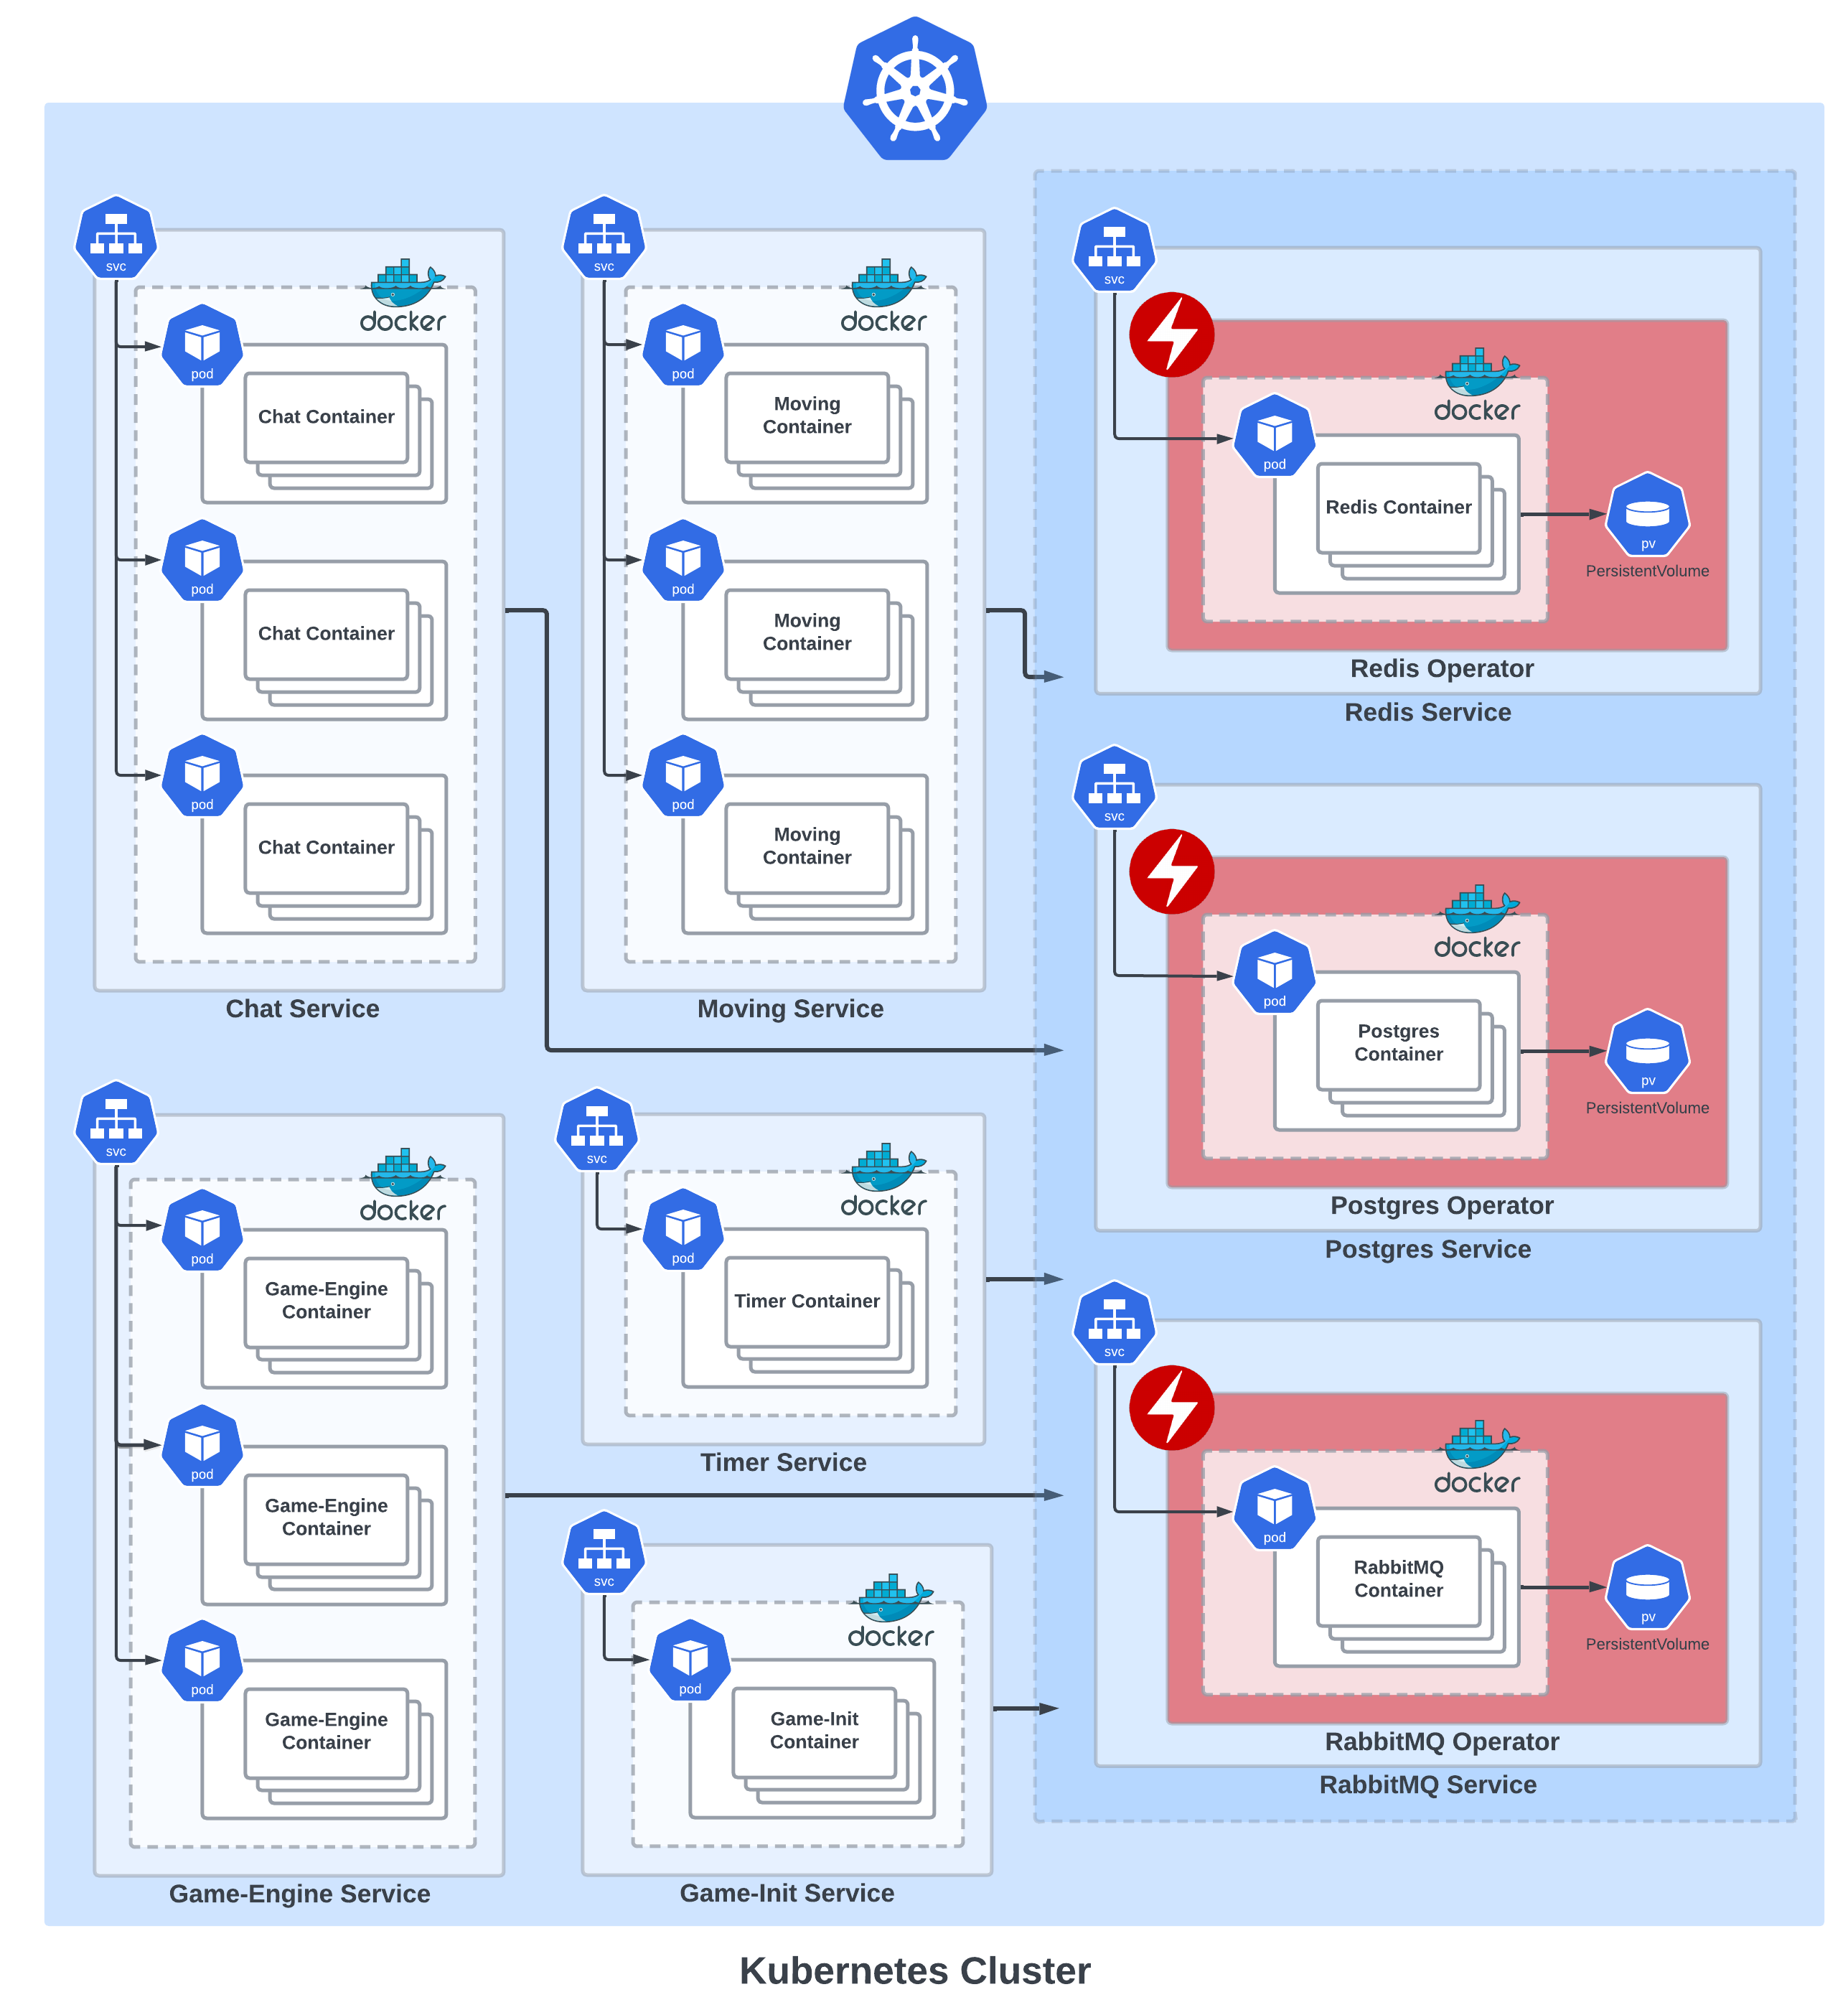
\includegraphics[width=0.9\linewidth]{resources/architecture_diagram.png}
    \caption{Diagram architektury rozwiązania z wykorzystaniem Kubernetesa}
    \label{fig:architecture}
\end{figure}

%%%%%%%%%%%%%%%%%%%%%%%%%%%%%%%%%%%%%%%%%%%%%%%%%%%%%%%%%%%%%%%%%%%%%%%%%%%%%%%
\chapter{Konfiguracja środowiska}
\label{sec:konfiguracja-srodowiska}

\section{Konfiguracja w Docker Compose}

Jako punkt wyjścia konfiguracji projektu został wyznaczony zmodyfikowany plik \texttt{docker-compose.yml}, za pomocą którego uruchamiane było middleware dla aplikacji backendowych oraz aplikacja webowa. Plik ten został rozszerzony o backendowe mikroserwisy oraz dodano wstępną konfigurację dla PostgreSQL, oraz RabbitMQ:

\begin{lstlisting}[caption=Przykład pliku Dockerfile dla mikroserwisu]
FROM gradle:7-jdk11 AS build
COPY .. /home/gradle/ecsb-backend
WORKDIR /home/gradle/ecsb-backend
RUN gradle :ecsb-chat:buildFatJar --no-daemon

FROM openjdk:11-jre-slim
EXPOSE 2138
WORKDIR /app
COPY --from=build /home/gradle/ecsb-backend/ecsb-chat/build/libs/*.jar /app/ecsb-chat.jar
ENTRYPOINT ["java", "-jar", "/app/ecsb-chat.jar"]
\end{lstlisting}

\begin{lstlisting}[caption=Przykładowa definicja kontenera mikroserwisu w pliku docker-compose.yml]
  moving:
    container_name: moving
    image: michwoj01/ecsb:moving
    build:
      context: ecsb-backend
      dockerfile: ./ecsb-moving/Dockerfile
    depends_on:
      - postgres
      - redis
      - rabbitmq
    restart: on-failure
    ports:
      - '8085:8085'
    networks:
      - my_network
\end{lstlisting}
\newpage

Przy okazji konfiguracji w Docker Compose pojawił się problem w postaci bardzo długiego budowania obrazów serwisów eCSB (ponad 6 minut), dlatego, uwzględniając fakt, że może się zmienić jedynie ich konfiguracja, założyliśmy repozytorium na DockerHub, gdzie wrzuciliśmy wszystkie obrazy eCSB, aby były dostępne do pobrania dla wszystkich członków zespołu. Przy okazji odchudziliśmy bazowe obrazy (openjdk:11 -> openjdk:11-jre-slim).

\begin{figure}[!htbp]
    \centering
    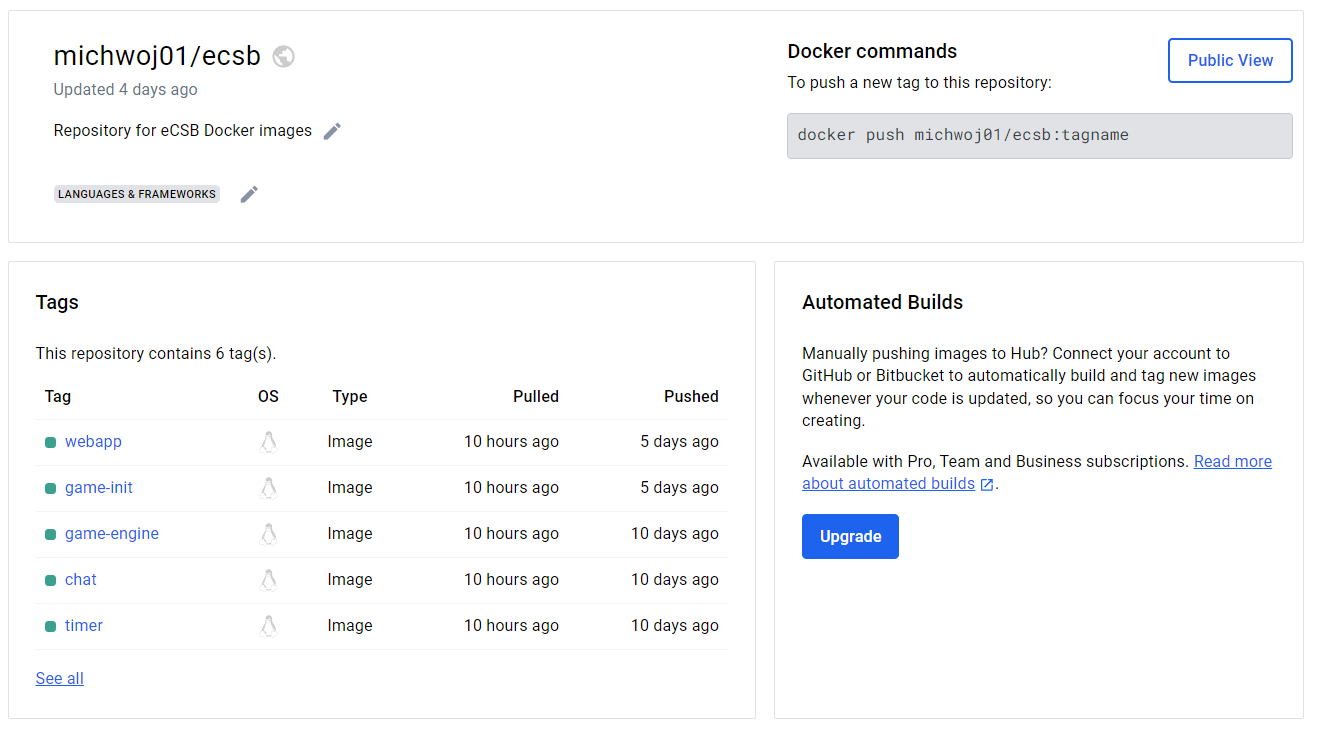
\includegraphics[width=0.9\linewidth]{resources/docker_hub.PNG}
    \caption{Repozytorium obrazów na DockerHub}
    \label{fig:dockerhub}
\end{figure}

\section{Konfiguracja w Kubernetes}
Mając z grubsza zdefiniowane kontenery składające się na architekturę, następnym krokiem było opakowanie ich w Kubernetesowe serwisy oraz konfiguracja zmiennych środowiskowych. 

W celu przeniesienia konfiguracji do Kubernetes należało stworzyć odpowiednie pliki YAML definiujące zasoby takie jak ConfigMap, Pod, Deployment, Service oraz PersistentVolumeClaim. Przykładowe pliki konfiguracyjne:

\subsection{Pod dla mikroserwisu}

\begin{lstlisting}[caption=Pod dla mikroserwisu]
apiVersion: v1
kind: Pod
metadata:
  name: chat
  labels:
    app.kubernetes.io/name: chat
spec:
  containers:
    - image: michwoj01/ecsb:chat
      name: chat
      ports:
        - containerPort: 2138
  restartPolicy: OnFailure
\end{lstlisting}

\subsection{Deployment dla PostgreSQL}

\begin{lstlisting}[caption=Deployment dla PostgreSQL]
apiVersion: apps/v1
kind: Deployment
metadata:
  name: postgres-operator
  namespace: default
spec:
  replicas: 1
  selector:
    matchLabels:
      app.kubernetes.io/name: postgres-operator
  template:
    metadata:
      labels:
        app.kubernetes.io/name: postgres-operator
    spec:
      serviceAccountName: postgres-operator-sa
      containers:
        - name: operator
          image: matipl01/ecsb-postgres-operator:v1.0.0
          ports:
            - containerPort: 5432
          args:
            - "--zap-log-level=debug"
            - "--zap-stacktrace-level=info"
            - "--zap-encoder=console"
\end{lstlisting}

\subsection{Service dla PostgreSQL}

\begin{lstlisting}[caption=Service dla PostgreSQL]
apiVersion: v1
kind: Service
metadata:
  name: postgres
spec:
  ports:
    - protocol: TCP
      port: 5432
      targetPort: 5432
  selector:
    app: postgres
\end{lstlisting}

\subsection{PersistentVolumeClaim dla PostgreSQL}

\begin{lstlisting}[caption=PersistentVolumeClaim dla PostgreSQL]
apiVersion: v1
kind: PersistentVolumeClaim
metadata:
  name: postgres-data-pvc
  namespace: default
  labels:
    app.kubernetes.io/name: postgres
spec:
  storageClassName: local-storage
  accessModes:
    - ReadWriteOnce
  resources:
    requests:
      storage: 1Gi
\end{lstlisting}

Konfiguracja w Kubernetes pozwala na zarządzanie mikroserwisami w bardziej skalowalny i elastyczny sposób, umożliwiając dynamiczne skalowanie, zarządzanie stanem aplikacji oraz łatwiejszą integrację z innymi komponentami systemu. Wszystkie pliki konfiguracyjne YAML powinny być umieszczone w odpowiednim katalogu (np. \texttt{kubernetes}), aby można było łatwo zastosować je w klastrze Kubernetes.

\section{Operator Framework dla middleware}
TODO

\section{Napotkane problemy}
\par Jednymi z najistotniejszych elementów konfiguracji poza zwykłym zdefiniowaniem plików YAMLowych okazały się:
\begin{itemize}
    \item skrypty bazodanowe — Postgres oprócz tworzenia i obsługi instancji wymagał dostępu do skryptów bazodanowych, które tworzyły wszystkie potrzebne tabele. Oprócz zamontowania wolumenów w klastrze Minikube potrzebne było również przekopiowanie samych skryptów do środka klastra, aby pody mogły z nich korzystać przy inicjalizacji. Niestety okazało się, że ten sposób przekazania skryptów nie może być zautomatyzowany, stąd skorzystaliśmy z przekształcenia skryptów do ConfigMap i przekazania ich jako parametry startowe podów Postgresa.
    \item dane Postgresa i Redisa — persystencja na lokalnym klastrze nie jest najlepszym rozwiązaniem (jeśli Minikube odmówi posłuszeństwa, dane przepadną), niemniej pojedyncze pody bywają jeszcze bardziej zawodne. Zamontowanie wolumenów zarówno dla danych statycznych (Postgres) jak i dynamicznych (Redis) było oczywistością.
    \item konfiguracja RabbitMQ — okazało się, że przekazanie plików konfiguracyjnych poprzez zamontowanie ConfigMap spowodowało błędy poda (oczywiście nigdzie nielogowane), które uniemożliwiały podłączenie się serwisów. Konieczne stało się w tym przypadku zastosowanie Operator Framework, aby inicjalizować pody RabbitMQ z odpowiednimi pluginami.
    \item zasoby potrzebne do stworzenia gry — jeden z modułów Chłopskiej Szkoły Biznesu wymagał zapisywania oraz odczytywania plików .jpg, będących elementami mapy lub grafikami postaci. Również w tym przypadku konieczne było zastosowanie persystentnego wolumenu wewnątrz klastra.
\end{itemize}

%%%%%%%%%%%%%%%%%%%%%%%%%%%%%%%%%%%%%%%%%%%%%%%%%%%%%%%%%%%%%%%%%%%%%%%%%%%%%%%
\chapter{\ChapterTitleInstallMethod} \label{sec:instalacja}

\section{Instalacja niezbędnych narzędzi}

\begin{enumerate}
  \item \textbf{Instalacja Docker}:
  \begin{enumerate}
    \item Należy przejść na stronę \href{https://www.docker.com/products/docker-desktop}{Docker Desktop} i pobrać odpowiednią wersję dla systemu operacyjnego (Windows, macOS, Linux).
    \item Następnie należy postępować zgodnie z opisanymi krokami instalacji dla używanego systemu operacyjnego.
  \end{enumerate}
  \item \textbf{Instalacja Minikube}:
  \begin{enumerate}
    \item Należy przejść na stronę \href{https://minikube.sigs.k8s.io/docs/start/}{Minikube} i pobrać odpowiednią wersję dla systemu operacyjnego, a następnie postępować zgodnie z krokami instalacji opisanymi w na załączonej stronie internetowej.
    \item Uruchomienie Minikube:
\begin{lstlisting}[basicstyle=\ttfamily, numbers=none]
minikube start\end{lstlisting}\vspace{-20pt}
  \end{enumerate}
\end{enumerate}

\section{Uruchomienie aplikacji na Kubernetes}

\begin{enumerate}
  \item \textbf{Pobranie repozytorium z rozwiązaniem}:
  \begin{lstlisting}[basicstyle=\ttfamily, numbers=none]
 git clone git@github.com:michwoj01/EOSI-Operator-Framework.git
 cd EOSI-Operator-Framework\end{lstlisting}\vspace{-20pt}
  \item \textbf{Zastosowanie wszystkich plików konfiguracyjnych Kubernetes oraz Custom Resource Definition}:
  \begin{lstlisting}[basicstyle=\ttfamily, numbers=none]
 cd kubernetes && ./deploy.sh\end{lstlisting}\vspace{-20pt}
  Jeżeli napotkano błąd \texttt{error looking up service account default/default: serviceaccount "default" not found}, należy ponownie uruchomić powyższą komendę.
  \item \textbf{Sprawdzenie statusu stworzonych elementów}:
  \begin{lstlisting}[basicstyle=\ttfamily, numbers=none]
kubectl get all\end{lstlisting}\vspace{-20pt}
\end{enumerate}

\section{Debugowanie}

W przypadku problemów, sprawdzenie statusu lub logów podów:
\begin{quote}
\begin{lstlisting}[basicstyle=\ttfamily, numbers=none]
kubectl describe <pod-name>
kubectl logs <pod-name>
\end{lstlisting}
\end{quote}

%%%%%%%%%%%%%%%%%%%%%%%%%%%%%%%%%%%%%%%%%%%%%%%%%%%%%%%%%%%%%%%%%%%%%%%%%%%%%%%
\chapter{\ChapterTitleSolutionSteps}
\label{sec:odtworzenie}

W tym rozdziale opisany jest proces odtworzenia całego rozwiązania krok po kroku, z wykorzystaniem podejścia Infrastructure as Code (IaC). Podejście to znacząco ułatwia proces wdrażania infrastruktury, poprzez jego automatyzację i ogranicza się do wykonania kilku komend, które, na podstawie zdefiniowanych plików konfiguracyjnych, wykonają niezbędną pracę za nas.

\section{Infrastructure as Code (IaC) - Podejście}

Infrastructure as Code (IaC) to praktyka zarządzania infrastrukturą IT przy użyciu kodu, co pozwala na automatyzację procesów wdrożeniowych oraz łatwe zarządzanie środowiskiem. W naszym projekcie wykorzystujemy Kubernetes do zarządzania kontenerami oraz Docker do budowy obrazów kontenerów. W celu zapewnienia infrastruktury dla naszego rozwiązania skorzystaliśmy z lokalnego klastra Minikube, w związku z czym nie było potrzeby korzystać z narzędzi typu Terraform.

\section{Kroki odtworzenia rozwiązania}

\begin{enumerate}
    \item \textbf{Instalacja narzędzi}:
    Na wstępie należy zainstalować niezbędne narzędzia, takie jak Docker, Minikube oraz kubectl zgodnie z instrukcjami podanymi w rozdziale dotyczącym instalacji, a także pobrać repozytorium i uruchomić konfigurację projektu. Dokładniej opisane jest to w rozdziale \ref{sec:instalacja}.

    \item \textbf{Dostęp do aplikacji webowej}:
    Po poprawnym uruchomieniu wszystkich usług, aplikacja webowa powinna być dostępna. Minikube dostarcza polecenie, które pozwala na dostęp do usług zewnętrznych poprzez otwarcie odpowiednich portów:
\begin{lstlisting}[basicstyle=\ttfamily, numbers=none]
minikube service webapp\end{lstlisting}\vspace{-20pt}
Następnie powinien otworzyć się tunel między klastrem Minikube a naszym lokalnym hostem i serwis aplikacji webowej powinien być dostępny lokalnie pod wyszczególnionym portem:
\begin{figure}[!htbp]
    \centering
    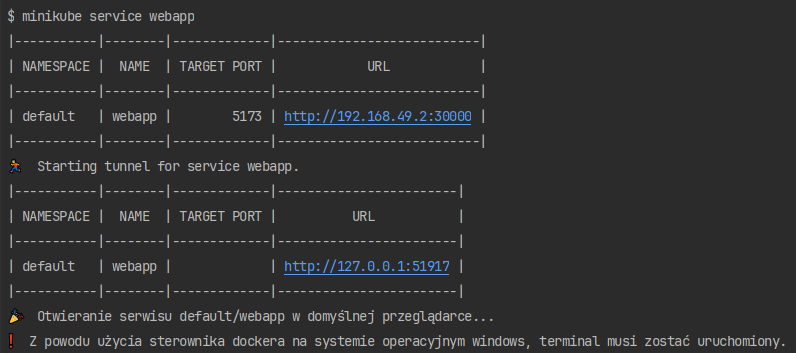
\includegraphics[width=0.9\linewidth]{resources/webapp expose.PNG}
    \caption{Otworzenie tunelu między Minikube a naszym hostem}
    \label{fig:tunel}
\end{figure}
\newpage
    \item \textbf{Zmiana liczebności skalowalnych serwisów}:
    Każdy serwis eCSB, który dzięki zastosowaniu shardingu jest możliwy do skalowania, możemy kontrolować za pomocą deklaracji Deploymentów. Dla przykładu możemy zwiększyć liczbę podów serwisu moving zmieniając parametr ilości replik:
\begin{figure}[!htbp]
    \centering
    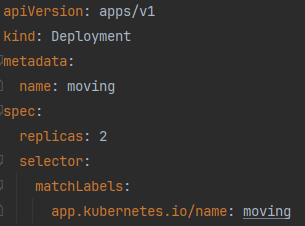
\includegraphics[width=0.6\linewidth]{resources/moving_replicas.PNG}
    \caption{Zmiana liczby podów serwisu moving}
    \label{fig:scaling}
\end{figure} 
    \item \textbf{Dostosowywanie się middleware do obciążenia}:
     Użycie Operator Framework do kontroli Postgresa umożliwia tworzenie replik jego instancji w miarę zwiększania się ilości serwisów (pojedyncza instancja Postgres ma ograniczoną liczbę dozwolonych połączeń):
    TODO
\end{enumerate}

%%%%%%%%%%%%%%%%%%%%%%%%%%%%%%%%%%%%%%%%%%%%%%%%%%%%%%%%%%%%%%%%%%%%%%%%%%%%%%%
\chapter{\ChapterTitleDemoDeployment}
\label{sec:deployment}
Mając środowisko minikube i aplikację w Kubernetes, dla odpowiednich serwisów (PostgreSQL, Redis, RabbitMQ) wprowadzeni zostali operatorzy utworzeni przy użyciu Operator Framework bazującym na Go.

\begin{enumerate}
    \item \textbf{Utworzenie repozytorium Operatora}: \verb|operator-sdk| automatycznie generuje projekt z bazowymi plikami do modyfikacji
    \begin{lstlisting}[basicstyle=\ttfamily, numbers=none]
 $ operator-sdk init\end{lstlisting}
\vspace{-20pt}
   \item \textbf{Stworzenie API oraz kontrolera}:
   również jest generowany bazowy kod dla resource API oraz kontrolera, np. dla PostgreSQL są to - \verb|postgres_types.go| oraz \verb|postgres_controller.go|, które następnie są dostosowywane do pożądanej funkcjonalności.
   \begin{lstlisting}[basicstyle=\ttfamily, numbers=none]
$ operator-sdk create api \
    --version=v1 \\end{lstlisting}

%     \begin{lstlisting}[caption=fragment kontrolera dla PostgreSQL]
% type Postgres struct {
% 	metav1.TypeMeta   `json:",inline"`
% 	metav1.ObjectMeta `json:"metadata,omitempty"`

% 	Spec   PostgresSpec   `json:"spec,omitempty"`
% 	Status PostgresStatus `json:"status,omitempty"`
% }
%     \end{lstlisting}
    
   Controller (kontroler) jest częścią Kubernetesa gdzie znajduje się logika Operatora. Za każdym razem gdy pojawia się jakaś zmiana na obserwowanym zasobie, funkcja \verb|Reconcile| ma doprowadzić aby aktualny stan CR (CustomResource) odpowiadał pożądanemu stanowi systemu. Dodatkowo, dzięki funkcji \verb|SetupWithManager()| zarządzamy zasobami pod kontrolerem oraz konfiguracjami.

    \begin{figure}[H]
        \centering
        \includegraphics[width=0.75\linewidth]{image.png}
        \caption{Schemat działania kontrolera\cite{hausenblas2019programming}}
        \label{fig:enter-label}
    \end{figure}
   
    \begin{lstlisting}[caption=fragment kontrolera dla PostgreSQL]
    func (r *PostgresReconciler) Reconcile(ctx context.Context, req ctrl.Request) (ctrl.Result, error) {
    	// Create a logger with context specific to this reconcile loop
    	logger := r.Log.WithValues("namespace", req.Namespace, "postgres", req.Name)
    	logger.Info("Reconciling Postgres instance")
    
    	// Fetch the Postgres instance
    	logger.Info("Fetching Postgres instance")
    	postgres := &databasev1.Postgres{}
    	err := r.Get(ctx, req.NamespacedName, postgres)
    	if err != nil {
    		if errors.IsNotFound(err) {
    			logger.Info("Postgres resource not found. Ignoring since object must be deleted")
    			return ctrl.Result{}, nil
    		}
    		logger.Error(err, "Failed to get Postgres")
    		return ctrl.Result{}, err
    	}
    
    	// Ensure PVCs exist
    	if err := r.ensurePVC(ctx, postgres.Spec.DataPvcName, postgres); err != nil {
    		logger.Error(err, "Failed to ensure data PVC")
    		return ctrl.Result{}, err
    	}
    
    	// Check if the Pod already exists
    	logger.Info("Checking if the Pod already exists")
    	found := &corev1.Pod{}
    	err = r.Get(ctx, types.NamespacedName{Name: postgres.Name, Namespace: postgres.Namespace}, found)
    	if err != nil && errors.IsNotFound(err) {
    		logger.Info("Pod does not exist, will create a new one")
    		// Define a new Pod object
    		logger.Info("Defining a new Pod object")
    		pod := r.newPodForCR(postgres)
    
    		// Set Postgres instance as the owner and controller
    		if err := controllerutil.SetControllerReference(postgres, pod, r.Scheme); err != nil {
    			logger.Error(err, "Failed to set controller reference")
    			return ctrl.Result{}, err
    		}
    
    		err = r.Create(ctx, pod)
    		if err != nil {
    			logger.Error(err, "Failed to create new Pod", "Pod.Namespace", pod.Namespace, "Pod.Name", pod.Name)
    			return ctrl.Result{}, err
    		}
    		// Pod created successfully - return and requeue
    		logger.Info("Pod created successfully")
    		return ctrl.Result{Requeue: true}, nil
    	} else if err != nil {
    		logger.Error(err, "Failed to get Pod")
    		return ctrl.Result{}, err
    	} else {
    		// If the Pod exists and is not managed by this operator, delete it
    		if !metav1.IsControlledBy(found, postgres) {
    			logger.Info("Found existing Pod not managed by this operator, deleting it", "Pod.Namespace", found.Namespace, "Pod.Name", found.Name)
    			err = r.Delete(ctx, found)
    			if err != nil {
    				logger.Error(err, "Failed to delete existing Pod", "Pod.Namespace", found.Namespace, "Pod.Name", found.Name)
    				return ctrl.Result{}, err
    			}
    			logger.Info("Deleted existing Pod", "Pod.Namespace", found.Namespace, "Pod.Name", found.Name)
    			return ctrl.Result{Requeue: true}, nil
    		}
    		logger.Info("Pod already exists and is managed by this operator", "Pod.Namespace", found.Namespace, "Pod.Name", found.Name)
    	}
    
    	// Update the Postgres status with the pod names
    	logger.Info("Updating Postgres status with the pod names")
    	podNames := []string{found.Name}
    	if !reflect.DeepEqual(podNames, postgres.Status.Nodes) {
    		postgres.Status.Nodes = podNames
    		err := r.Status().Update(ctx, postgres)
    		if err != nil {
    			logger.Error(err, "Failed to update Postgres status")
    			return ctrl.Result{}, err
    		}
    		logger.Info("Postgres status updated", "Status.Nodes", postgres.Status.Nodes)
    	}
    
    	return ctrl.Result{}, nil
    }
\end{lstlisting}


\item \textbf{Utworzenie CRD}: wygenerowanie CustomResourceDefinition, który Operator ma obserwować oraz nim zarządzać
\begin{lstlisting}[basicstyle=\ttfamily, numbers=none]
$ make manifests\end{lstlisting}
% \end{enumerate}

\begin{lstlisting}[caption=Fragment CRD dla PostgreSQL]
---
apiVersion: apiextensions.k8s.io/v1
kind: CustomResourceDefinition
metadata:
  annotations:
    controller-gen.kubebuilder.io/version: v0.13.0
  name: postgres.database.pl.edu.agh
spec:
  group: database.pl.edu.agh
  names:
    kind: Postgres
    listKind: PostgresList
    plural: postgres
    singular: postgres
  scope: Namespaced
  versions:
  - name: v1
    schema:
      openAPIV3Schema:
        description: Postgres is the Schema for the postgres API
        properties:
          apiVersion:
            description: 'APIVersion defines the versioned schema of this representation
              of an object. Servers should convert recognized schemas to the latest
              internal value, and may reject unrecognized values. More info: https://git.k8s.io/community/contributors/devel/sig-architecture
              /api-conventions.md#resources'
            type: string
          kind:
\end{lstlisting}

\item \textbf{Uruchomienie Operatora}: lokalnie, przy podłączeniu do klastra Kubernetes
\begin{lstlisting}[basicstyle=\ttfamily, numbers=none]
$ make install run\end{lstlisting}
% \end{enumerate}

    
\end{enumerate}

Po utworzeniu odpowiednich Operatorów oraz ich wdrożeniu na klastrze minikube można obserwować ich działanie dla naszego scenariusza \ref{scenario}.


...


[skriny scenariusza]
%%%%%%%%%%%%%%%%%%%%%%%%%%%%%%%%%%%%%%%%%%%%%%%%%%%%%%%%%%%%%%%%%%%%%%%%%%%%%%%
\chapter{\ChapterTitleSummary}
\label{sec:podsumowanie}

Operator Framework to przydatne narzędzie do orch

%%%%%%%%%%%%%%%%%%%%%%%%%%%%%%%%%%%%%%%%%%%%%%%%%%%%%%%%%%%%%%%%%%%%%%%%%%%%%%%

\section{Rysunki, tabele}
\label{sec:rysunki-tabele}

\subsection{Rysunki}
\label{sec:rysunki}

Przykładowy odnośnik do rysunku~\ref{fig:ex1}.

\begin{figure}[!htbp]
  \centering
\includegraphics[width=.7\textwidth]{resources/example.pdf}
\caption[Przykładowy rysunek]{Przykładowy rysunek (źródło:
  \cite{author2021title})}
\label{fig:ex1}
\end{figure}
 
W przypadku rysunków można odwoływać się zarówno do poszczególnych części
składowych --- rysunek~\ref{fig:sub1} i rysunek~\ref{fig:sub2}) --- jak i do
całego rysunku~\ref{fig:ex2}.

\begin{figure}[!htbp]
\begin{center}
\subfigure[Tytuł 1]{%
\label{fig:sub1}
\includegraphics[width=0.48\textwidth]{resources/example.pdf}}%
\subfigure[Tytuł 2]{%
\label{fig:sub2}
\includegraphics[width=0.48\textwidth]{resources/example.pdf}}
\end{center}
\caption[Kolejne przykładowe rysunki]{Kolejne przykładowe rysunki (źródło:
  \cite{author2021title})}
\label{fig:ex2}
\end{figure}

%%%%%%%%%%%%%%%%%%%%%%%%%%%%%%%%%%%%%%%%%%%%%%%%%%%%%%%%%%%%%%%%%%%%%%%%%%%%%%% 

\section{Cytowania}
\label{sec:cytowania}

Przykład cytowania literatury~\cite{wilson2009prediction-interday}. Kolejny przykład
cytowania kilku pozycji bibliograficznych~\cite{allen1999using-genetic, zitzler1999evolutionary-algorithms, pictet1995genetic-algorithms, wilhelmstotter2021jenetics, chmaj2015DistributedProcessingApplications}.
%%%%%%%%%%%%%%%%%%%%%%%%%%%%%%%%%%%%%%%%%%%%%%%%%%%%%%%%%%%%%%%%%%%%%%%%%%%%%%%
\section{Listy}
\label{sec:listy}

Lista z elementami:
\begin{itemize}
\item pierwszym,
\item drugim,
\item trzecim.
\end{itemize}

Lista numerowana z dłuższymi opisami:
\begin{enumerate}
\item Pierwszy element listy.
\item Drugi element listy.
\item Trzeci element listy.
\end{enumerate}
%%%%%%%%%%%%%%%%%%%%%%%%%%%%%%%%%%%%%%%%%%%%%%%%%%%%%%%%%%%%%%%%%%%%%%%%%%%%%%%

\printbibliography

%%%%%%%%%%%%%%%%%%%%%%%%%%%%%%%%%%%%%%%%%%%%%%%%%%%%%%%%%%%%%%%%%%%%%%%%%%%%%%%
\listoffigures
\listoftables
\listofalgorithmes
\lstlistoflistings

\end{document}
